% Chapter 1

\chapter{Introducción general} % Main chapter title

\label{Chapter1} % For referencing the chapter elsewhere, use \ref{Chapter1} 


%----------------------------------------------------------------------------------------
%	SECTION 1
%----------------------------------------------------------------------------------------
Este capítulo introduce al lector a los procesos de prueba de temporizadores y drivers de LEDs y las diferentes opciones disponibles. También se presentan los objetivos y el alcance establecido. 

\label{IntroGeneral}

%----------------------------------------------------------------------------------------

% Define some commands to keep the formatting separated from the content 
\newcommand{\keyword}[1]{\textbf{#1}}
\newcommand{\tabhead}[1]{\textbf{#1}}
\newcommand{\code}[1]{\texttt{#1}}
\newcommand{\file}[1]{\texttt{\bfseries#1}}
\newcommand{\option}[1]{\texttt{\itshape#1}}
\newcommand{\grados}{$^{\circ}$}

%----------------------------------------------------------------------------------------

%\section{Introducción}

%----------------------------------------------------------------------------------------
\section{Contexto}

La industria manufacturera es aquella que se dedica a la transformación de la materia prima en bienes de consumo. Además de procesos de transformación de materia, se desarrollan otros en simultáneo, muchos de ellos asociados a la gestión de la calidad. La industria de la manufactura electrónica no es ajena a estos procesos y en particular dentro de aquellos que hacen a la calidad, hay uno muy importante que es la prueba final del producto. Esta consiste principalmente en la verificación de su correcto funcionamiento y del cumplimiento de sus especificaciones. Para estas pruebas es común el uso de instrumentos y dispositivos de prueba diseñados específicamente para un tipo o una familia de productos en particular.

La empresa Posthac S.A., la cual impulsó el desarrollo del sistema que trata esta memoria, cuenta con una amplia línea de productos en el área de iluminación automática e iluminación para vía pública, de los cuales hay dos grupos que se destacan: los temporizadores y los drivers para luminarias LED. La razón que destaca estos productos es que los primeros son los de mayor volumen de venta dentro de los que se producen en las instalaciones de la empresa, y los segundos son productos que están en etapa de desarrollo y con amplia perspectiva de venta en el área de iluminación de vía pública.
Ante esta situación se realizó un relevamiento de la capacidad actual de la empresa, principalmente en lo que se refiere a prueba de productos, y se evaluaron distintas opciones de mejora que se detallarán a continuación.


%\subsection{Temporizadores para iluminación}
\section{Temporizadores para iluminación}

Un temporizador para iluminación es un dispositivo semiautomático que tiene como función principal mantener encendida una luminaria durante un tiempo preestablecido luego de recibir un pulso de activación, normalmente generado con un pulsador. Estos dispositivos son de uso común en viviendas y edificios. En la actualidad los temporizadores electrónicos son los de mayor difusión, pero existen otros tipos como los temporizadores mecánicos.

Dentro de los temporizadores electrónicos los hay de dos, tres y cuatro terminales de conexión, de tiempo fijo o ajustable y con salidas conmutadas por relé o triac. En la figura \ref{fig:TGE} se observa un temporizador con salida a rele de cuatro teminales, mientras que la figura \ref{fig:TQLED} es de un temporizador con pulsador de tres terminales. La principal diferencia entre ambos es que los temporizadores de cuatro terminales poseen una entrada de activación independiente y los de tres terminales se activan por el mismo terminal que se sirve de salida.

\begin{figure}[htbp]
  \centering
  \begin{subfigure}[b]{0.47\textwidth}
    \centering
     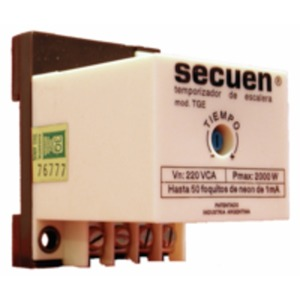
\includegraphics[width=0.8\textwidth]{./Figures/TGE.jpg}
	\caption{\protect\raggedright Temporizador de cuatro terminales.}
	\label{fig:TGE}
  \end{subfigure}
  \hfill
  \begin{subfigure}[b]{0.47\textwidth}
    \centering
     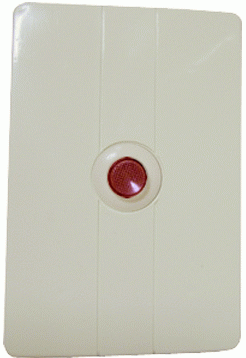
\includegraphics[width=0.55\textwidth]{./Figures/TQLED.png}
	\caption{\protect\raggedright Temporizador de tres terminales.}
	\label{fig:TQLED}
  \end{subfigure}
	\caption{Temporizadores para iluminación de uso residencial}
    \label{fig:three graphs}
\end{figure}


La prueba de este tipo de dispositivo consiste en verificar los siguientes puntos:

\begin{itemize}
	\item Accionamiento correcto de la carga.
	\item Cumplimiento de tiempo de encendido máximo.
	\item Cumplimiento de tiempo de encendido mínimo.
\end{itemize}

En el momento de hacer la evaluación, las pruebas de temporizadores en la empresa las hacía un operario utilizando un cronómetro y el banco de pruebas de la figura \ref{fig:Probador}, donde se podían conectar hasta seis temporizadores a la vez. Usando estos elementos el operario verificaba los puntos antes indicados en forma manual.

\begin{figure}[ht]
	\centering
	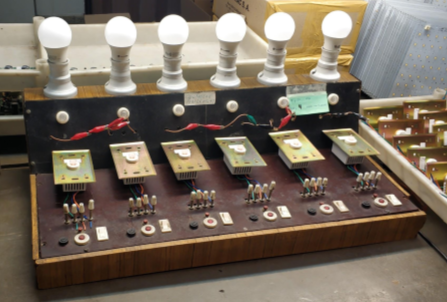
\includegraphics[scale=.7]{./Figures/Probador.png}
	\caption{Probador de temporizadores.}
	\label{fig:Probador}
\end{figure}

Dado que estos productos no tienen un nivel de producción y venta muy masivo, no se encuentran opciones comerciales de sistemas automáticos de prueba. Incluso grandes y medianas empresas en China, que el autor de esta memoria ha visitado, utilizan sistemas propios o métodos manuales para realizar estas pruebas.


%\subsection{Drivers para luminarias LED}
\section{Drivers para luminarias LED}

Los diodos LED son dispositivos semiconductores capaces de convertir la energía eléctrica en luz. Para que el LED funcione de forma adecuada y alcanzar la vida útil establecida, la excitación se debe realizar manteniendo la temperatura dentro del rango de trabajo. Esto se consigue utilizando algún medio para extraer el calor, como disipadores o forzadores, y limitando la potencia sobre los LEDs. Para lograr que la potencia sobre los LEDs sea estable y esté limi-
tada al rango de trabajo se utilizan los drivers de LED. Estos drivers son equipos que convierten la energía eléctrica a una forma adecuada para excitar las cargas LED. La característica principal de este tipo de drivers es que entregan en su salida una corriente constante, de modo que la potencia sobre los LEDs resulte estable. Además, muchos de estos drivers tienen la posibilidad de dimerizar o controlar la corriente de salida mediante una entrada adicional para dicho fin. Esta entrada de dimerizado permite controlar el nivel de iluminación producido por los LEDs y además posibilita controlar la temperatura de trabajo de los LED. Para tal fin, se utilizan sensores que miden y retroalimentan al driver la temperatura sobre los LEDs. Si es necesario, el driver reducirá la potencia entregada y así se bajará la temperatura.
En la figura \ref{fig:Driver} se puede ver un modelo de driver típico de luminarias LED para vía pública.

\begin{figure}[ht]
	\centering
	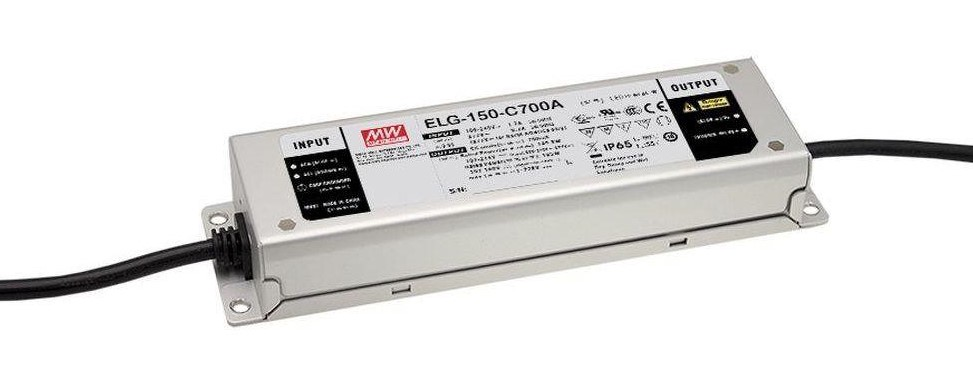
\includegraphics[scale=.6]{./Figures/Driver.jpg}
	\caption{Driver para LEDs.}
	\label{fig:Driver}
\end{figure}


En lo que respecta a la prueba de este tipo de equipos, los principales parámetros son:
\begin{itemize}
	\item Tensión de salida.
	\item Corriente de salida.
	\item Función de dimerizado si corresponde.
	\item Potencia de entrada.
	\item Factor de potencia.
\end{itemize}

	Para hacer estas pruebas existen en el mercado diferentes opciones  de equipamiento con distintas características. En la tabla \ref{tab:ProbadoresDrivers} se comparan algunos modelos evaluados, donde se puede apreciar que en general los sistemas de prueba de drivers están diseñados para probar de un equipo a la vez.
	
	\begin{table}[h]
	\centering
	\caption[Tabla de comparación de equipos de prueba de drivers]{Comparación de equipos de prueba de drivers}
	\begin{tabular}{l c c c c}    
		\toprule
		\textbf{Prueba} 	 & \textbf{63115A} & \textbf{61501}& \textbf{LT101A}		& \textbf{WT5080}  \\
		\midrule
		Factor de potencia & - & SÍ & SÍ & SÍ \\		
		Tensión de entrada	 & - & 0-500V & 3-300V & 1-500V \\
		Corriente de entrada& - & 0-30A & 10mA-5A & 5mA-5A \\
		Tensión de salida & 0-600V & - & 3-300V & 3-500V \\		
		Corriente de salida & 0-5A & - & 10mA-5A & 5mA-5A \\		
		Dimerizado & NO & NO & NO & NO \\		
		Emulación de Carga & SÍ & NO & NO & NO \\
		Pruebas simultáneas &2/4 & 1 & 1 & 1 \\
		Marca & Chroma & Chroma & Everfine & InvenFine \\
		\bottomrule
		\hline
	\end{tabular}
	\label{tab:ProbadoresDrivers}
\end{table}

\section{Motivación}

Luego de analizar las opciones disponibles para la prueba de temporizadores y drivers de LEDs, es evidente que para el caso de la prueba de temporizadores se requiere un sistema diseñado a medida. Además, si bien hay distintas opciones para pruebas de drivers de LED, ninguna de ellas cumple con la necesidad de la empresa Posthac S.A. de tener un sistema de pruebas adaptable a distintos productos y expandible para poder probar múltiples equipos al mismo tiempo. De este modo surgió la idea de desarrollar este sistema de pruebas que, además de satisfacer las necesidades actuales, deje lugar a futuras adaptaciones para distintas pruebas.

\section{Objetivos y alcance}
\subsection{Objetivos}
Los objetivos inicialmente propuestos para el trabajo realizado son: reducir los tiempos de prueba para lograr un uso eficiente de las horas hombre, mejorar la calidad de las pruebas y estar preparados para las futuras producciones de drivers de LED.
\subsection{Alcance}
El desarrollo se limitó a los siguientes puntos:
\begin{itemize}
	\item Desarrollo y fabricación del prototipo del módulo principal.
	\item Desarrollo y fabricación de prototipos de dos módulos adicionales. Uno para ensayo de 			temporizadores y otro para ensayo de salida de drivers para luminarias LED.
	\item Desarrollo de la interfaz de usuario mediante conexión WIFI.	
	\item Código fuente.
	\item Diagramas eléctricos y diseños de PCB.
\end{itemize}

No están incluidos:

\begin{itemize}
	\item Otros módulos adicionales no detallados anteriormente.
	\item Interfaz gráfica para la conexión mediante cable con PC.
\end{itemize}





